\chapter{Progettazione Logica} 

\section{Gerarchia}
La gerarchia della classe \textit{Persona} è stata implementata con partizionamento verticale visto che entrambe le sottoclassi \textit{Istruttore} e \textit{Socio} hanno degli attributi propri e considerato il fatto che sia la classe radice che le due sottoclassi hanno delle associazioni proprie.\\
Si è scelto di sostituire la generalizzazione con associazioni, in modo da evitare di avere attributi con valori nulli suul'entità genitore e di ridurre la dimensione delle entità figlie. 

\section{Descrizione testuale dello schema relazionale}
Le chiavi primarie vengono indicate come \underline{sottolineate}, mentre le chiavi esterne vengono marcate con un asterisco (*).\\

\begin{itemize}
\item \textsc{Persona}(\underline{\textbf{CodFiscale}}: string, \textbf{Nome} :string, \textbf{Cognome}: string, \textbf{DataNasc}: date,\\ \textbf{LuogoNasc}: string, \textbf{Telefono}: string,  \textbf{Mail}: string, \textbf{Sesso}: enum\{'Maschio', 'Femmina'\} ) 
\begin{itemize}
\item Tutti i campi di Persona sono implementati come NOT NULL (tranne telefono, perché facoltativo).
\end{itemize}

\item \textsc{Istruttore}(\underline{\textbf{CodFiscale}*}: string, \textbf{Qualifica}: string, \textbf{Retribuzione}: int, \textbf{DataAssunzione}: date)
\begin{itemize}
\item Tutti i campi sono NOT NULL tranne il campo \textit{Qualifica} che può essere vuoto.
\item \textit{Retribuzione} deve essere un valore positivo, maggiore di zero.
\end{itemize}

\item \textsc{Socio}(\underline{\textbf{CodFiscale}*}: string, \textbf{DataIscrizione}: date. \textbf{Livello}: enum\{'Principiante',\\'Intermedio','Esperto'\})  
\begin{itemize}
\item Tutti i campi sono NOT NULL.
\end{itemize}

\item \textsc{Account}(\underline{\textbf{CodFiscale}*} string, \textbf{UserName}: string, \textbf{Admin}: bool, \textbf{Hash}: string )
\begin{itemize}
\item Tutti i campi sono NOT NULL.
\item Il campo \textit{Admin} rappresenta i permessi e distingue un utente con permessi amministrativi (istruttore, 1) da un utente con permessi di default (socio, 0).
\item Il campo \textit{Hash} memorizza l'hash SHA1 della password associata all'account.
\end{itemize}

\item \textsc{Corso}(\underline{\textbf{CodCorso}*}: int, \textbf{NomeCorso}: string, \textbf{TipoCorso}: enum\{'Principiante',\\'Intermedio','Avanzato'\}, \textbf{Attivo}: bool, \textbf{CodFiscale}*: string)
\begin{itemize}
\item Tutti i campi tranne \textit{CodFiscale} sono NOT NULL. Vi possono essere corsi per il quale non v'è Istruttore.
\item Il campo \textit{Attivo} che determina se un corso è attivo, oppure no, è impostato di default a zero.
\end{itemize}
\item \textsc{Campo}(\underline{\textbf{CodCampo}}: int, \textbf{TipoSup}: enum\{'Terra Rossa','Erba Sintetica','PlayIt'\})
\begin{itemize}
\item Tutti i campi sono NOT NULL.
\end{itemize}

\item \textsc{Lezione}(\underline{\textbf{CodLezione}}: int, \underline{\textbf{CodCorso}*}: int )   
\item \textsc{IscrittoCorso}(\underline{CodCorso}*: int, \underline{\textbf{CodFiscale}*}: string) 
\begin{itemize}
\item Nuova tabella derivante dall'associazione \textit{IscrittoCorso}
\end{itemize}
\item \textsc{Prenotazione}(\textbf{CodCorso}*:int, \textbf{CodLezione}*: int, \textbf{CodFiscale}*: string, \underline{\textbf{CodCampo}*}: int, \underline{\textbf{Data}}: date, \underline{\textbf{Ora}}: tinyint)  
\begin{itemize}
\item I campi \textit{CodCorso}, \textit{CodLezione}, \textit{CodFiscale} possono essere NULL ma non tutti e tre contemporaneamente.
\end{itemize}
\end{itemize}

\section{Vincoli semantici non catturati dallo schema}
\section{Schema logico}
\begin{figure}[H]
 \centering
  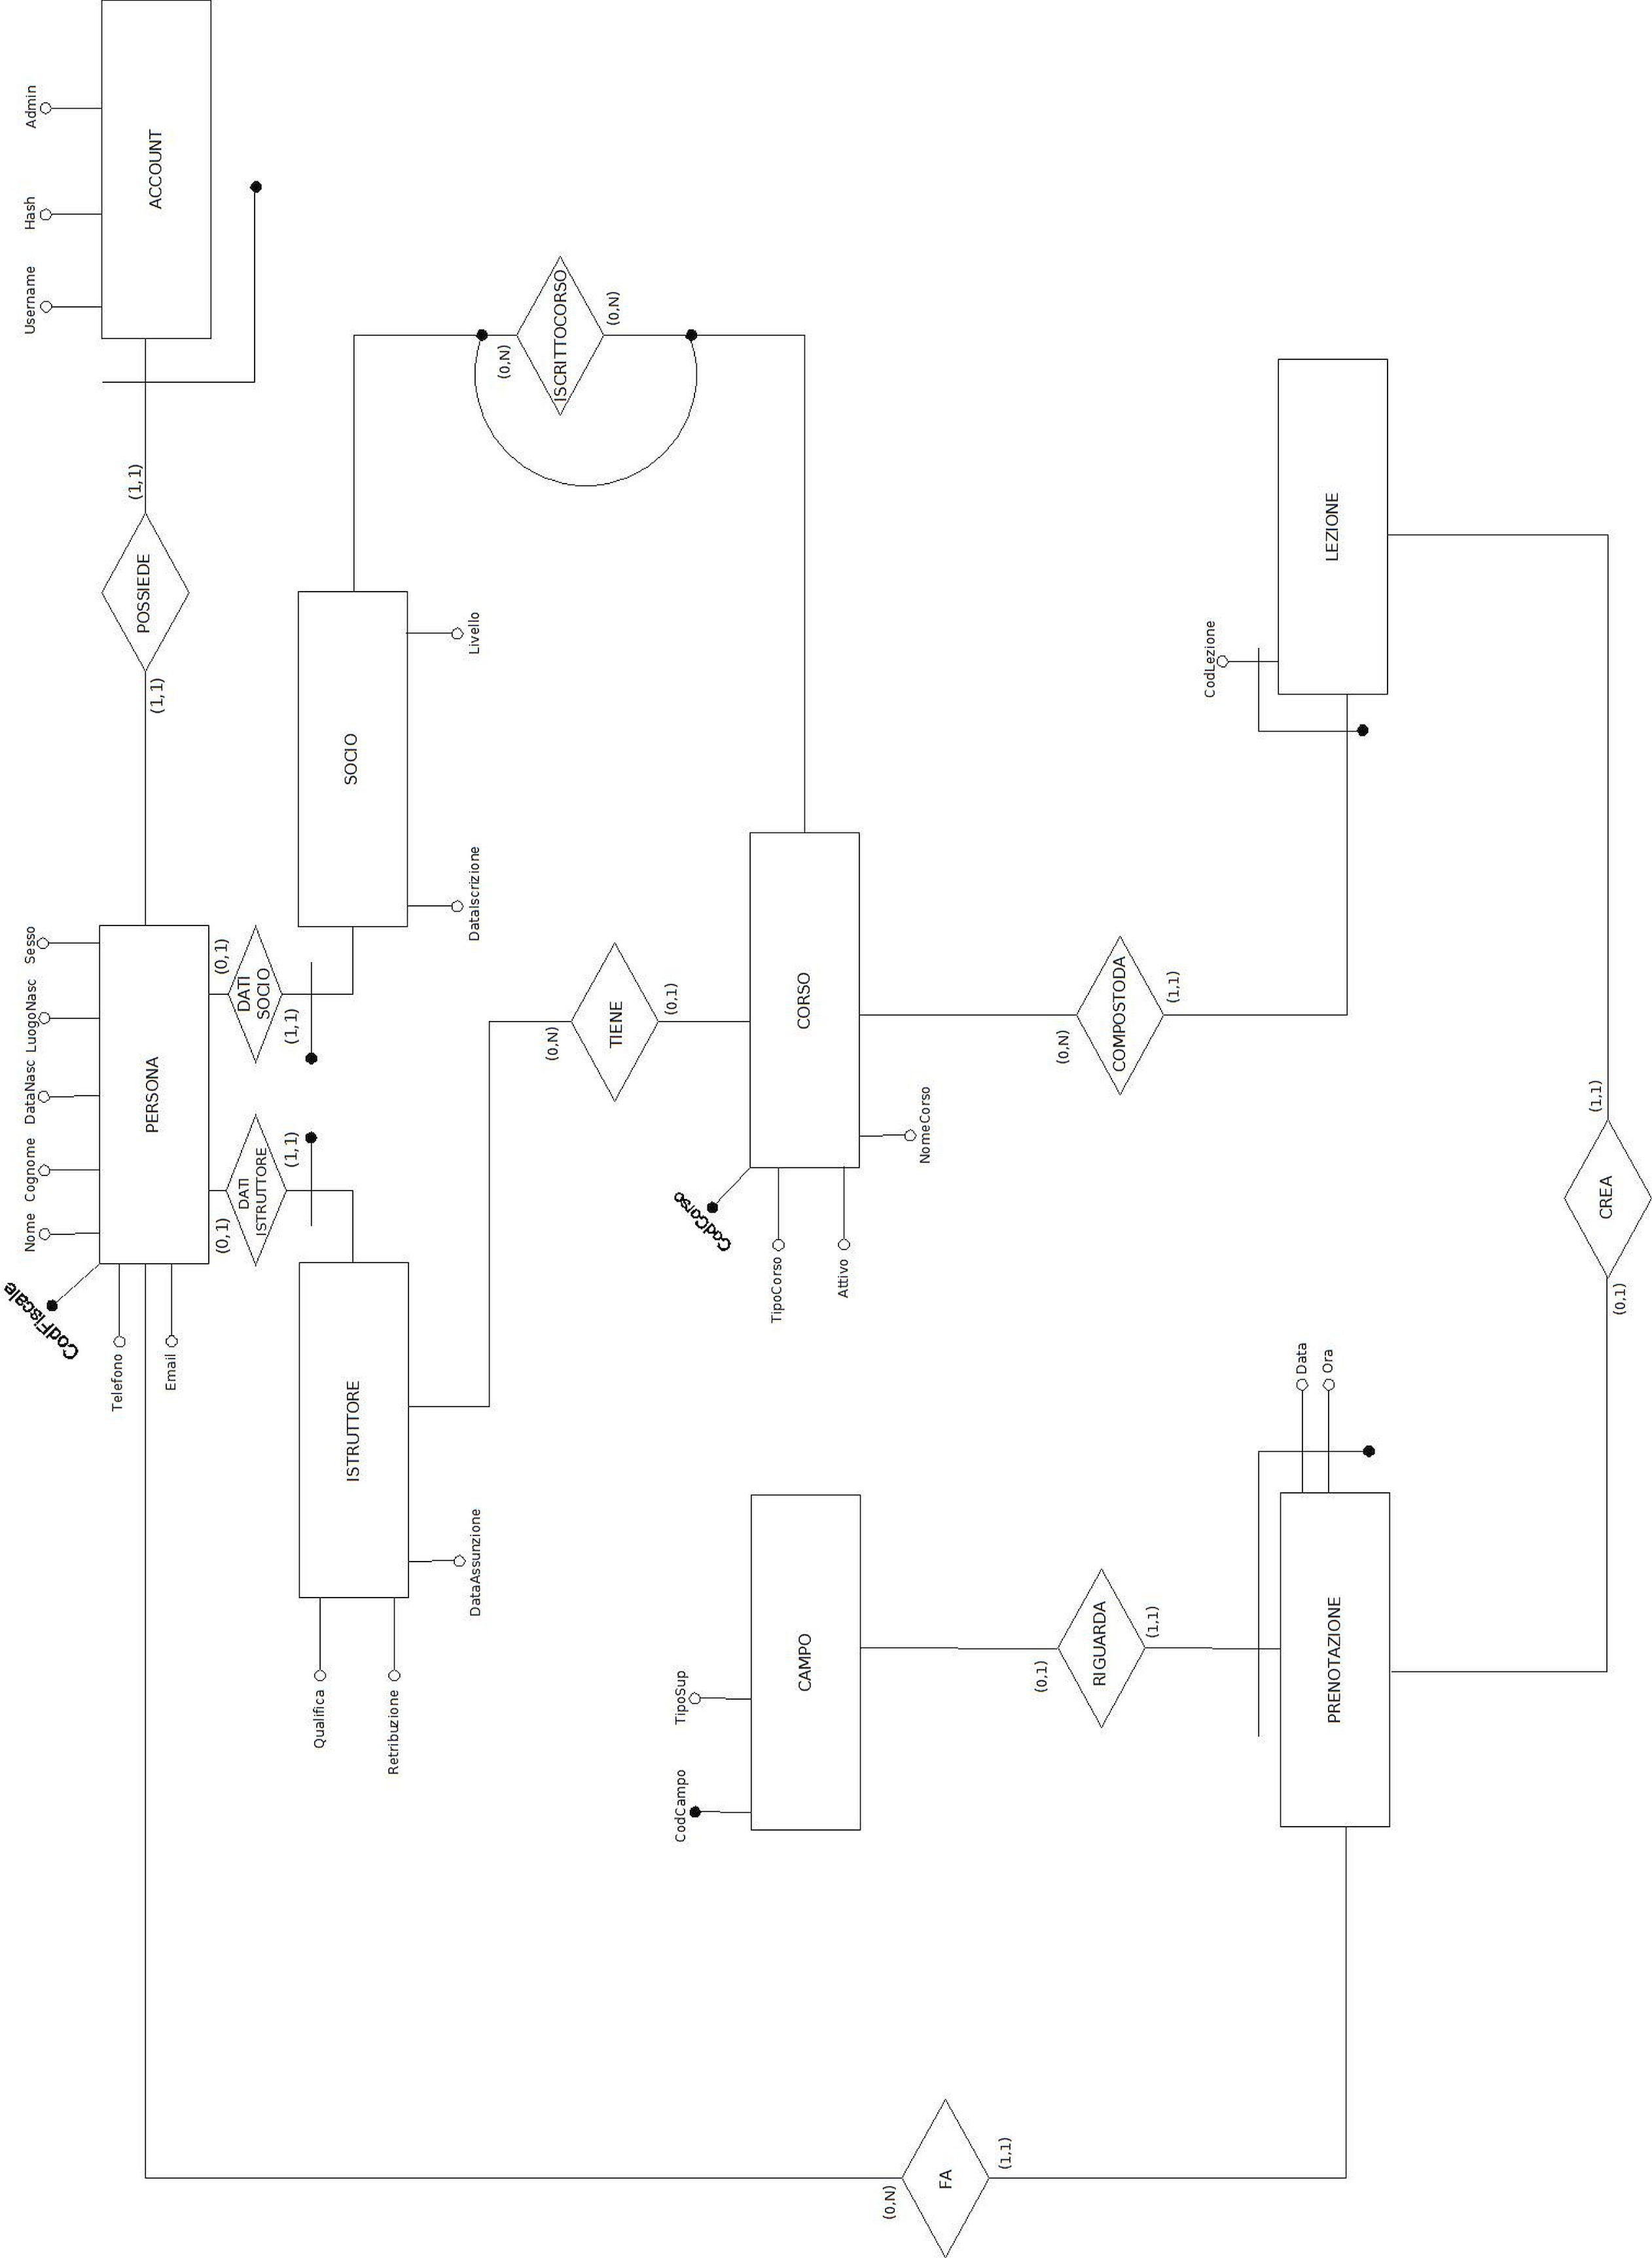
\includegraphics[width=\textwidth, height=\textheight]{Images/LOGICO.jpg}
\caption{Lo Schema Concettuale E-R Ristrutturato}
\end{figure}
\chapter{Implementazione dello schema logico tramite DDL di MySQL} 
\lstinputlisting[language=SQL]{sql/DDL_Database.sql}
